\documentclass{article}
\usepackage[T1]{fontenc}
\usepackage{lmodern}
\usepackage{graphicx}
\usepackage{amsmath,amssymb}
\usepackage[a4paper,margin=2cm]{geometry}
\usepackage[absolute,overlay]{textpos}
\setlength{\TPHorizModule}{1mm}
\setlength{\TPVertModule}{1mm}
\usepackage[indonesian]{babel}
\usepackage{hyperref}
\setlength{\emergencystretch}{2em}
% unit: Halaman 5

\begin{document}

% === Halaman 5 (llm) ===

\vspace{149.39mm}

Namun, dibalik sebuah gambar dapat tersembunyi informasi rahasia
\vspace{60mm}
Informasi rahasia tersebut dapat berupa pesan biasa, pesan kejahatan, program jahat, bahkan virus komputer!

% deskripsi: Ilustrasi steganografi yang menunjukkan gambar Mona Lisa dengan panah yang mengarah ke sekumpulan kode biner dan teks 'VIRUS', melambangkan penyembunyian data rahasia di dalam gambar.
% bbox normalisasi: [0.2480, 0.2300, 0.6830, 0.7330]
\begin{textblock*}{91.35mm}(52.08mm,68.31mm)
\noindent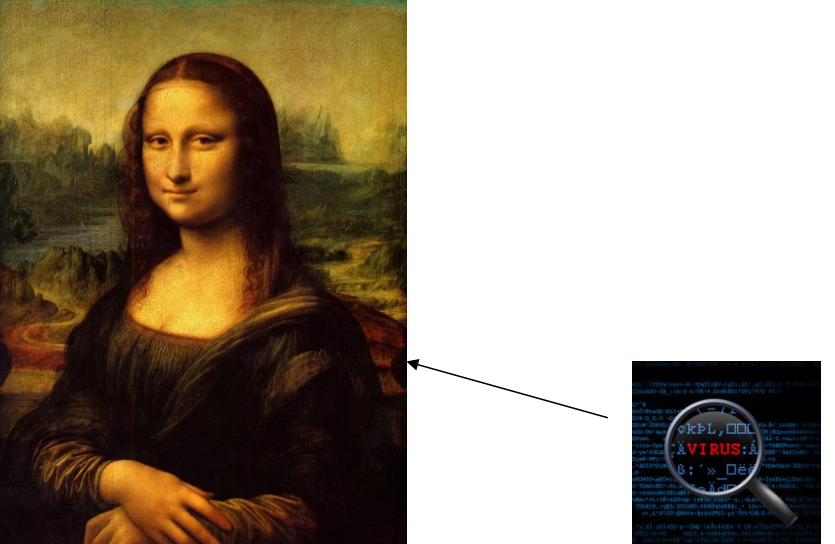
\includegraphics[width=91.35mm,height=149.39mm]{../../images/llm/page_005_img_01.png}%
\end{textblock*}

\end{document}
